\chapter{\textbf{Resultados}} % Este comando é utilizado para criar capítulos
\sloppy % Corrige estouro de linhas

\section{Aplicativo Mobile}

Todo o processo de construção do Web Service e do Aplicativo foi baseado na metodologia utilizada na disciplina de Laboratório de Engenharia de Software \cite{rupLes}. Para tanto, foram realizadas as seguintes etapas:

\subsection{Levantar Requisitos (Visão Geral)}

Nesta etapa foi realizado um levantamento de funcionalidades básicas necessárias junto a empresa responsável pelo gerenciamento dos dados dos alunos. A partir desta, foi elaborado uma descrição geral sobre o escopo do aplicativo.

\subsection{Elaborar Modelo Conceitual}

A construção do modelo conceitual foi baseada no levantamento realizado na etapa anterior, levando em consideração as informações disponibilizadas pela base de dados cedida, conforme a figura \ref{figura:modelo_conceitual}.

\begin{figure}[H]
	\caption{Modelo Conceitual.}
	\centering % para centralizarmos a figura
	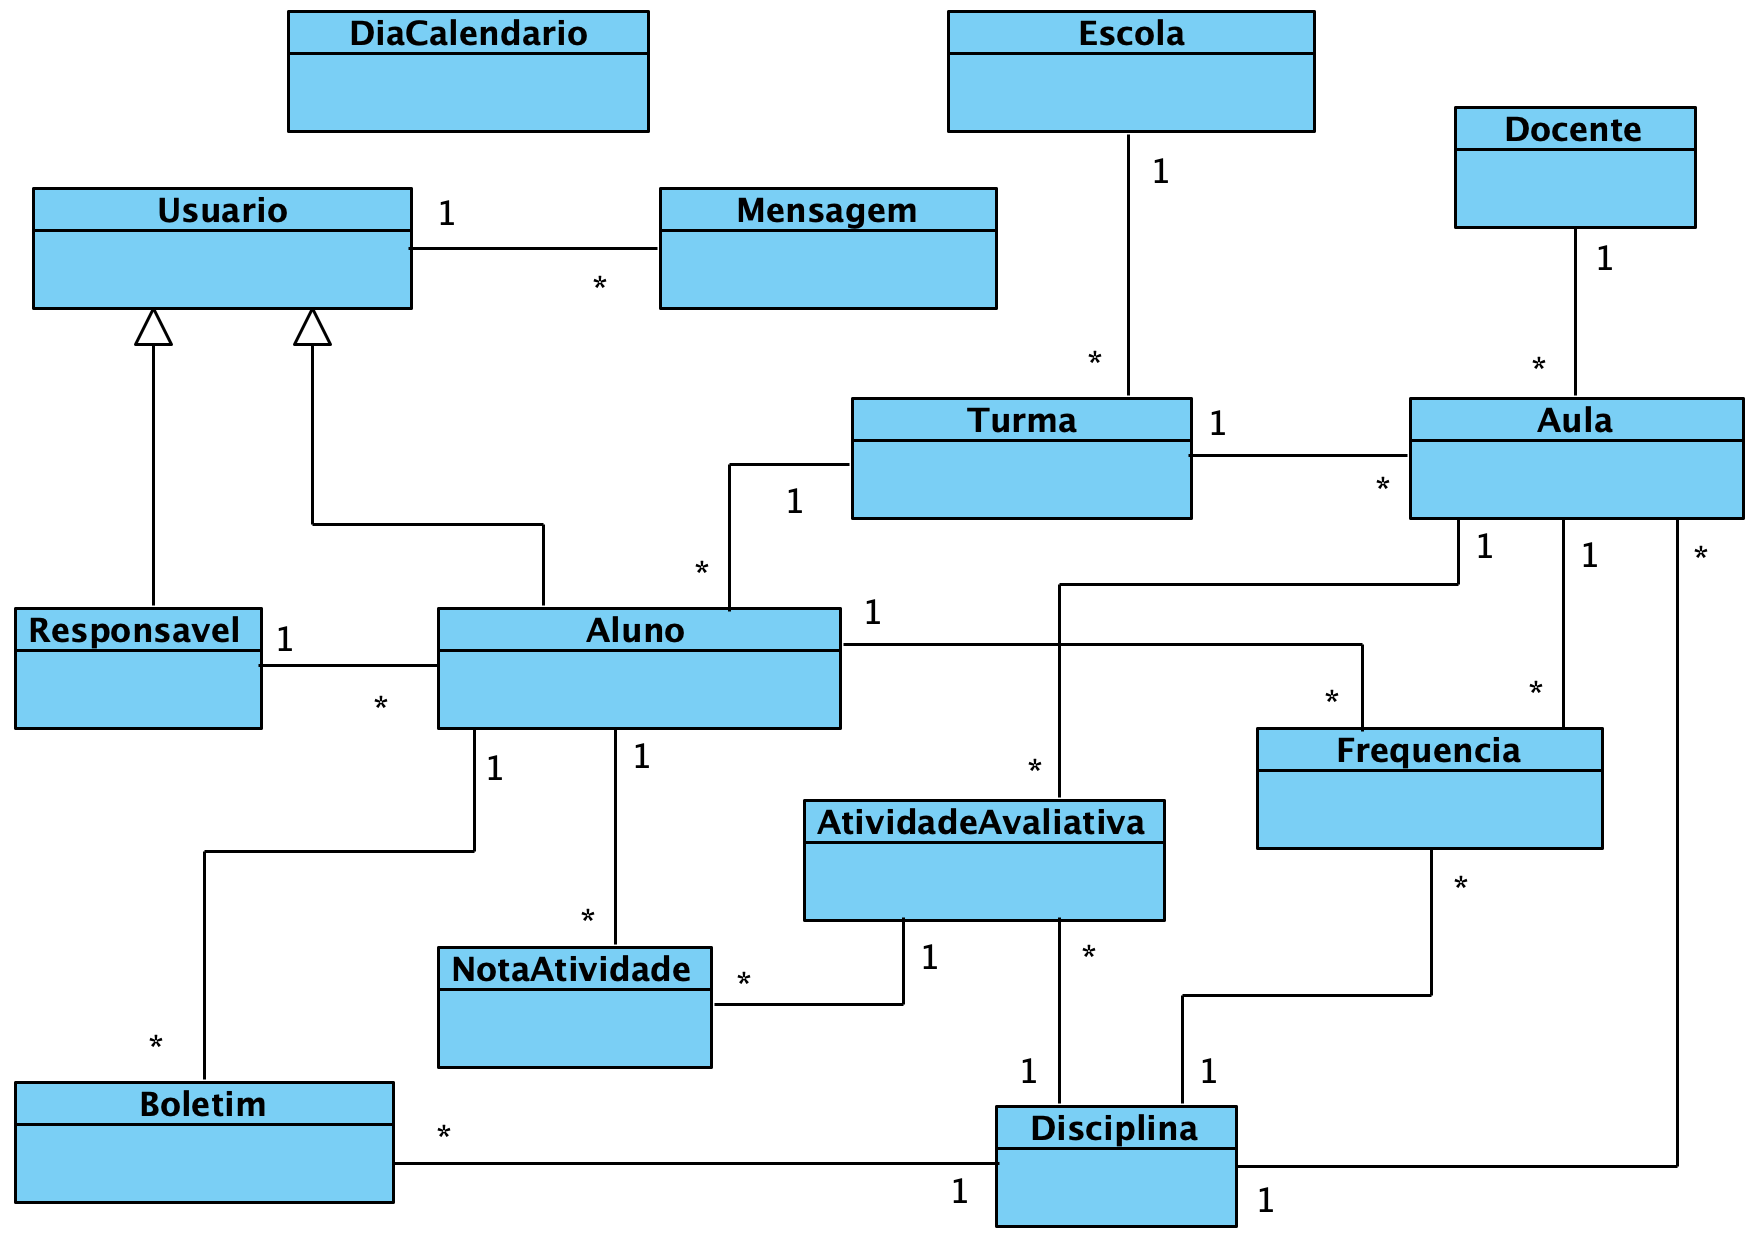
\includegraphics[width=15cm]{resources/modelo_conceitual.png} % leia abaixo
	\label{figura:modelo_conceitual}
	\footnotesize{\text{Fonte: O Autor.}}
\end{figure}

\subsection{Levantar Requisitos}

Nesta etapa foi produzido o documento de requisitos. Ao todo, foram identificados 12 requisitos, sendo 2 de processos de negócio e 10 de listagens. Todos os requisitos foram definidos a partir de reuniões realizadas com a empresa responsável por ceder os dados.

\subsection{Organizar Requisitos}

Nesta etapa, os requisitos forma organizados entre as categorias: processos de negócios e listagens/relatórios.

Os requisitos de processos de negócio foram, respectivamente: entrar no sistema e sair do sistema.

Os requisitos de listagem foram, respectivamente: listar alunos por responsável, listar grade horária por aluno, listar atividades avaliativas por aluno e trimestre, listar frequências por aluno, disciplina e trimestre, listar boletim por aluno e trimestre, listar dados do aluno, listar dados da emeb por aluno, listar mensagens por aluno, listar mensagens por responsável, listar calendário acadêmico.

% \begin{center}
%     \begin{table}[]
%         \centering
%         \caption{Caption}
%         \begin{tabular}{ c c c c }
%             \hline
%             col1 & col2 & col3 \\
%             \hline
%             \multirow{3}{4em}{Multiple row} & cell2 & cell3 \\ 
%             & cell5 & cell6 \\ 
%             & cell8 & cell9 \\ 
%         \hline
%         \end{tabular}
%         \label{tab:my_label}
%     \end{table}
% \end{center}

\subsection{Elaborar diagrama de classes de projeto}

Nesta etapa foi elaborado o diagrama de classes de projeto, considerando os dados a serem utilizados no aplicativo, levantados no documento de requisitos.

\begin{figure}[H]
	\caption{Diagrama de Classe.}
	\centering % para centralizarmos a figura
	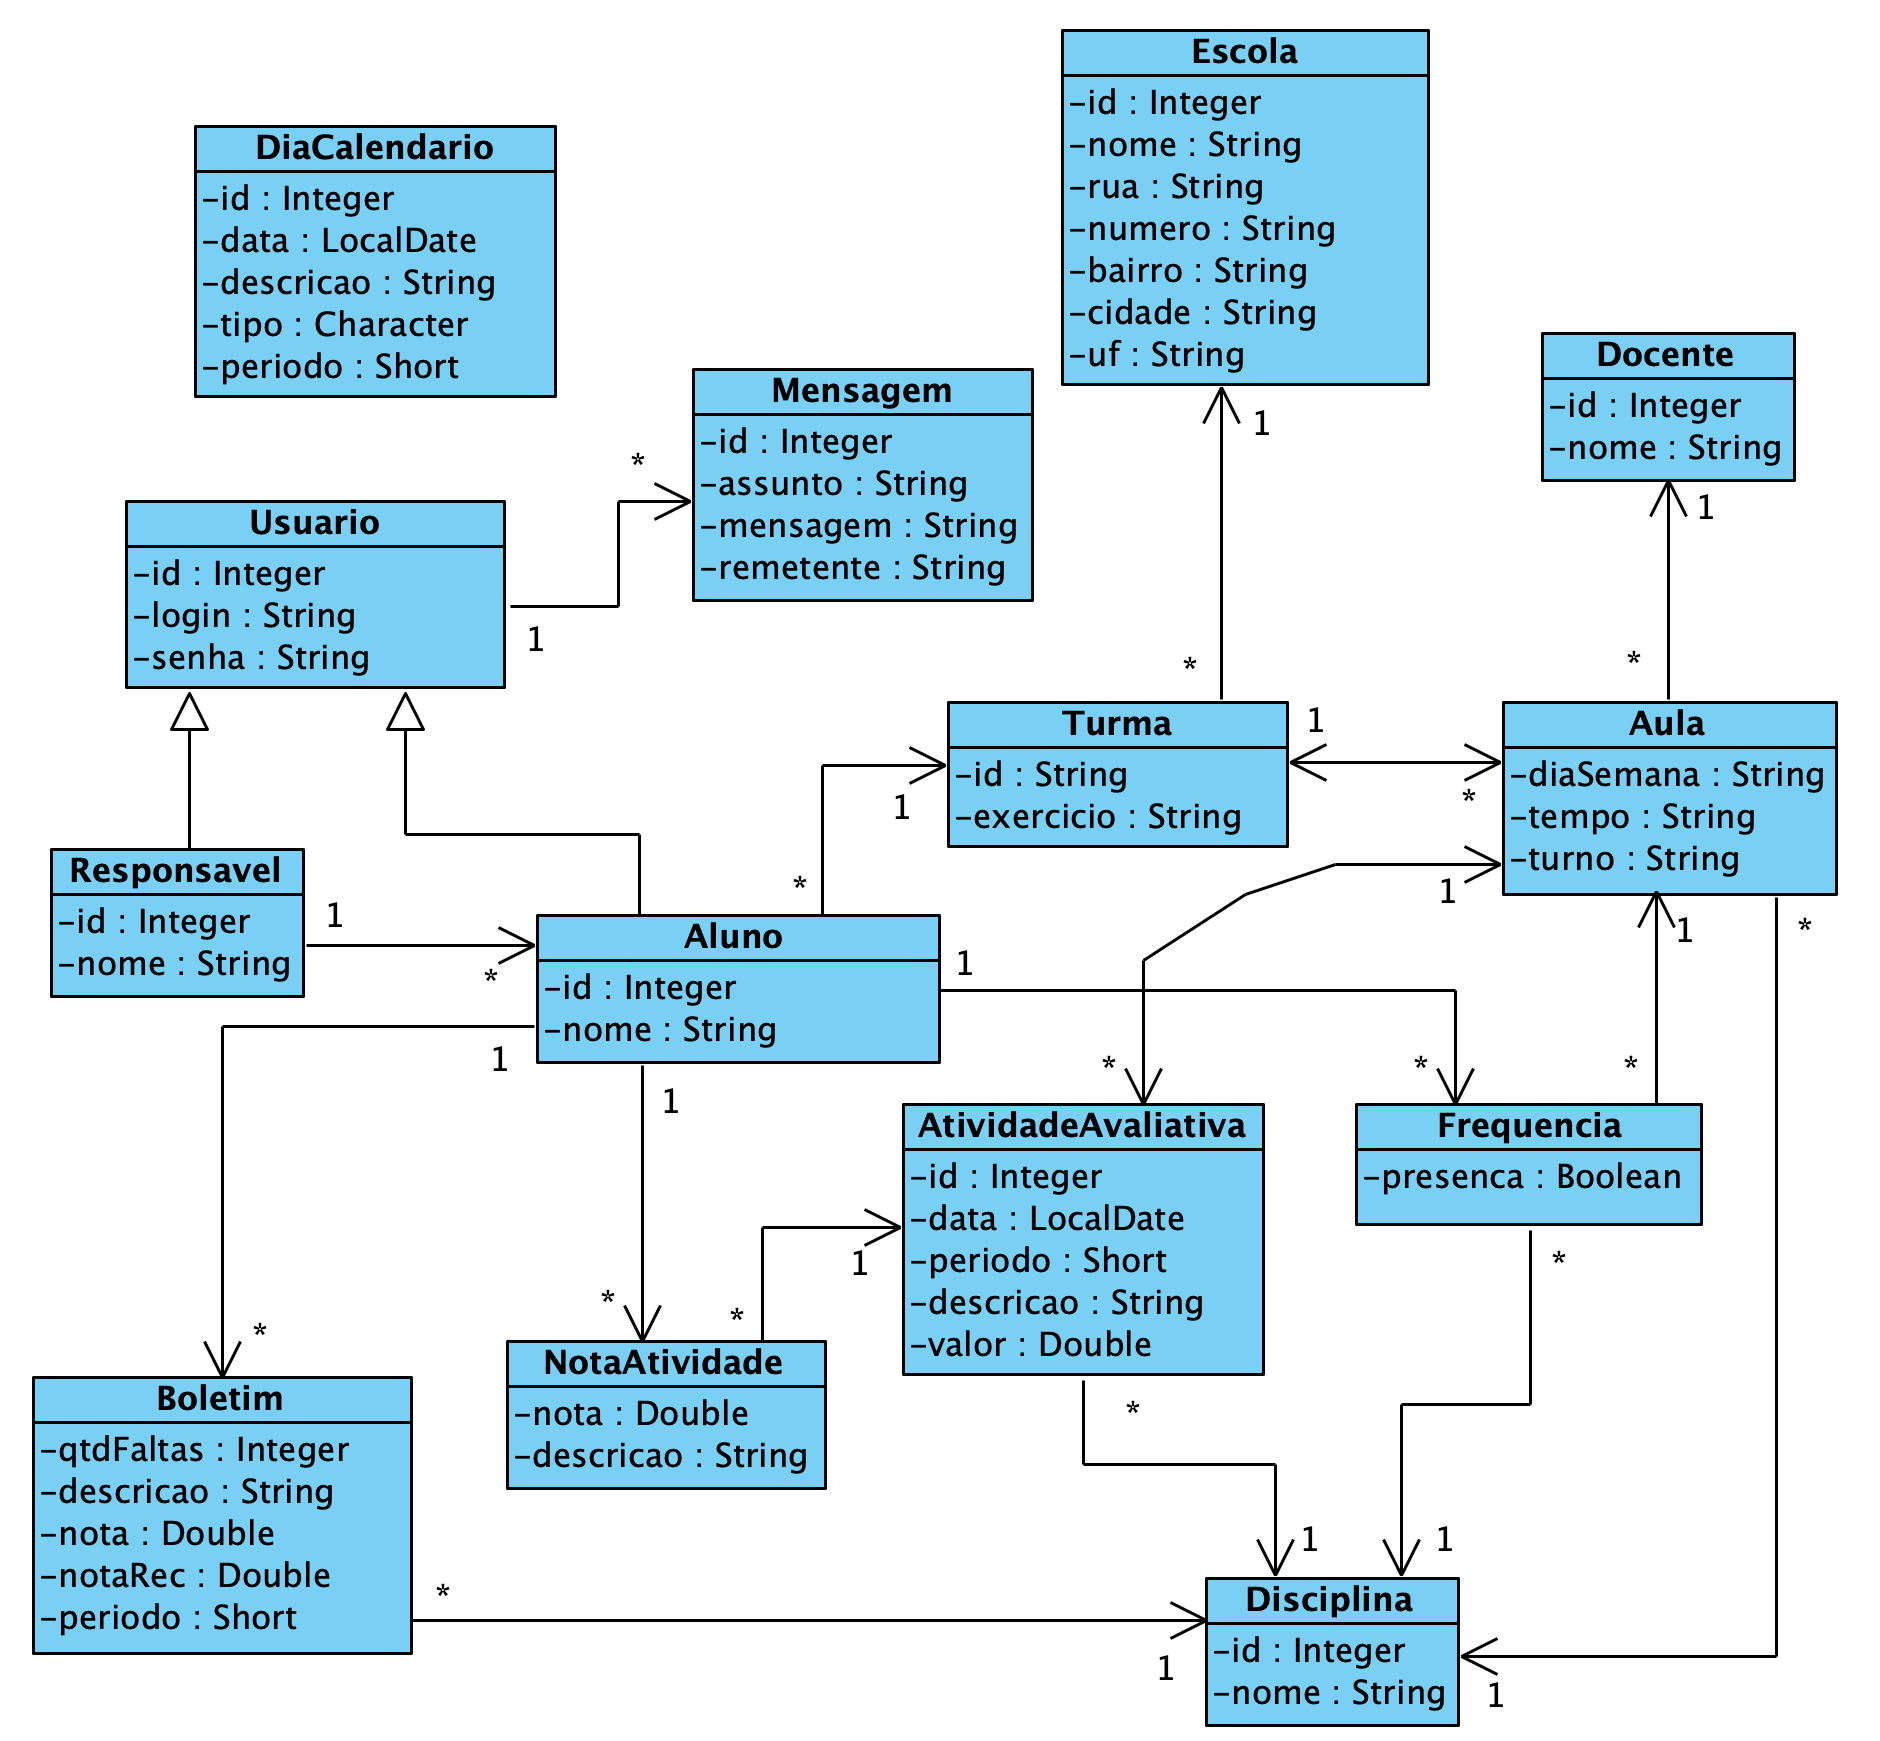
\includegraphics[width=16cm]{resources/classes_projeto.png} % leia abaixo
	\label{figura:diagrama_classe}
	\caption*{Fonte: O Autor.}
\end{figure}

\subsection{Implementar}

\subsubsection{Aplicativo Mobile}

O aplicativo mobile foi implementado utilizando a linguagem Typescript, através do \textit{framework} de desenvolvimento Ionic, na versão 4. A tabela \ref{tabela:app_organizacao} demonstra a organização básica dos principais diretórios do projeto, bem como suas respectivas descrições: 

\renewcommand{\arraystretch}{1.5}
\begin{table}[H]
	\centering
	\caption{Organização de Diretórios do Aplicativo Mobile.}
	\label{tabela:app_organizacao}
	\begin{tabular}{c l}
	    \hline
		\multicolumn{1}{l|}{\textbf{Diretório}} & \multicolumn{1}{c}{\textbf{Descrição}}\\
		\hline
		models & Classes de mapeamento de dados retornados pela API  \\
		pages & Telas do aplicativo \\
		services & Classes de acesso ao Web Service \\
		\hline
	\end{tabular}
	\caption*{Fonte: O Autor.}
\end{table}
\renewcommand{\arraystretch}{1}

A seguir serão apresentadas as telas implementadas para as funcionalidades definidas no escopo do projeto:

% \begin{figure}[h]
%     \caption{Tela de Login.}
% 	\centering % para centralizarmos a figura
% 	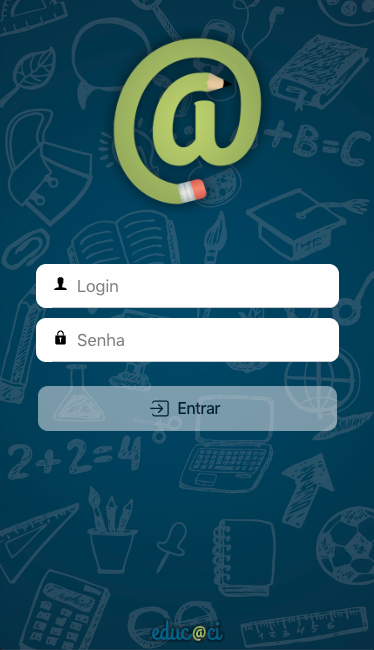
\includegraphics[width=6cm]{resources/prints_app/login.png} % leia abaixo
% 	\label{figura:login}
% 	\caption*{Fonte: O Autor.}
% \end{figure}

\begin{figure}[H]
    \begin{minipage}[b]{0.45\linewidth}
        \caption{Tela de Login.}
    	\centering % para centralizarmos a figura
    	\shadowbox{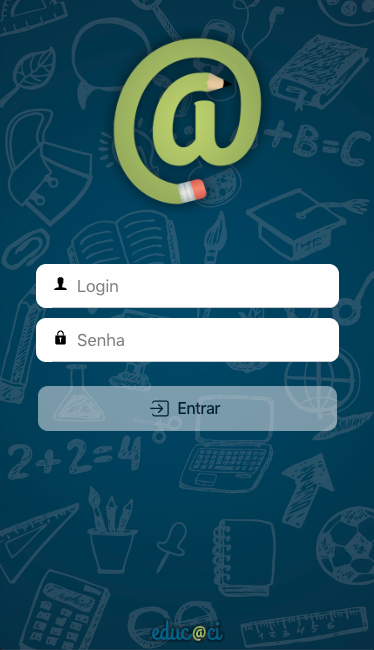
\includegraphics[width=6cm]{resources/prints_app/login.png}} % leia abaixo
    	\label{figura:login}
    	\caption*{Fonte: O Autor.}
    \end{minipage}
    \hspace{0.5cm}
    \begin{minipage}[b]{0.45\linewidth}
        \caption{Menu principal.}
    	\centering % para centralizarmos a figura
    	\shadowbox{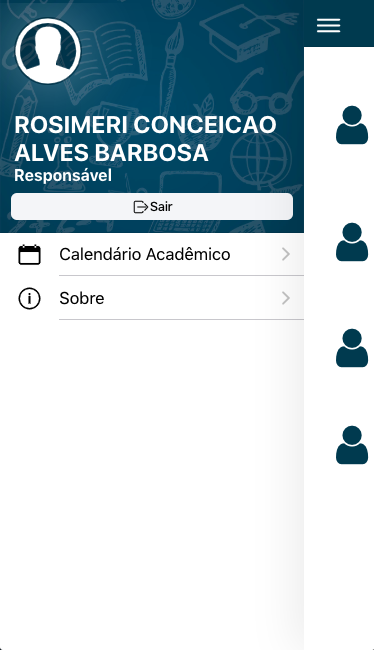
\includegraphics[width=6cm]{resources/prints_app/usuario_menu.png}} % leia abaixo
    	\label{figura:login}
    	\caption*{Fonte: O Autor.}
    \end{minipage}
\end{figure}

\begin{figure}[H]
    \begin{minipage}[b]{0.45\linewidth}
        \caption{Listagem de alunos.}
    	\centering % para centralizarmos a figura
    	\shadowbox{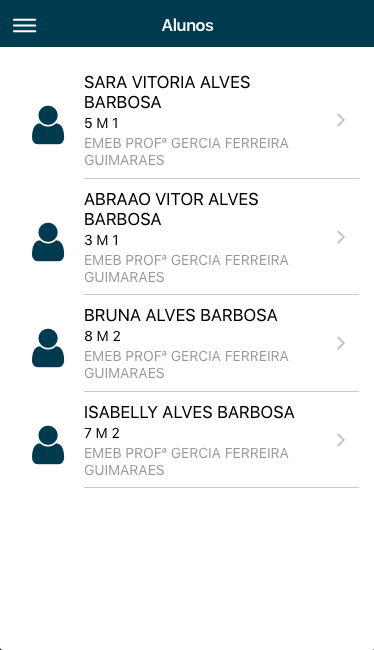
\includegraphics[width=6cm]{resources/prints_app/listagem_alunos.png}} % leia abaixo
    	\label{figura:login}
    	\caption*{Fonte: O Autor.}
    \end{minipage}
    \hspace{0.5cm}
    \begin{minipage}[b]{0.45\linewidth}
        \caption{Perfil de um aluno.}
    	\centering % para centralizarmos a figura
    	\shadowbox{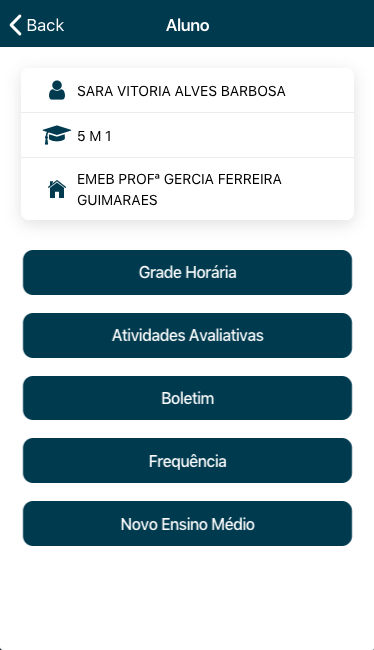
\includegraphics[width=6cm]{resources/prints_app/perfil_aluno.png}} % leia abaixo
    	\label{figura:login}
    	\caption*{Fonte: O Autor.}
    \end{minipage}
\end{figure}

\begin{figure}[H]
    \begin{minipage}[b]{0.45\linewidth}
        \caption{Listagem de dias da hrade horária.}
    	\centering % para centralizarmos a figura
    	\shadowbox{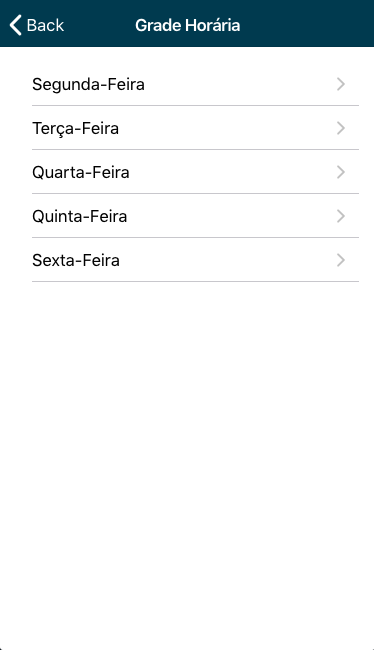
\includegraphics[width=6cm]{resources/prints_app/grade_horaria1.png}} % leia abaixo
    	\label{figura:login}
    	\caption*{Fonte: O Autor.}
    \end{minipage}
    \hspace{0.5cm}
    \begin{minipage}[b]{0.45\linewidth}
        \caption{Exibição do horário de aulas por dia da grade horária.}
    	\centering % para centralizarmos a figura
    	\shadowbox{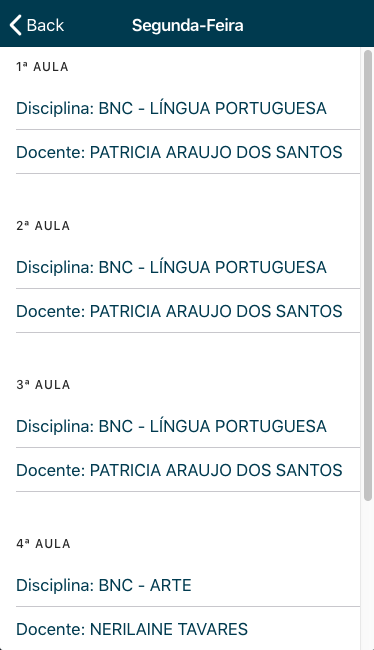
\includegraphics[width=6cm]{resources/prints_app/grade_horaria2.png}} % leia abaixo
    	\label{figura:login}
    	\caption*{Fonte: O Autor.}
    \end{minipage}
\end{figure}

\begin{figure}[H]
    \begin{minipage}[b]{0.45\linewidth}
        \caption{Listagem de atividades avaliativas.}
    	\centering % para centralizarmos a figura
    	\shadowbox{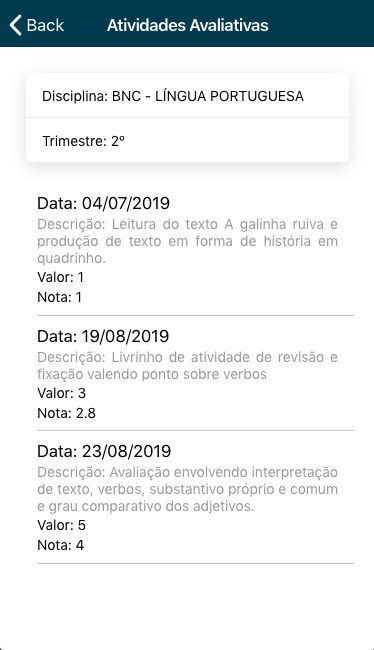
\includegraphics[width=6cm]{resources/prints_app/atividades_avaliativas.png}} % leia abaixo
    	\label{figura:login}
    	\caption*{Fonte: O Autor.}
    \end{minipage}
    \hspace{0.5cm}
    \begin{minipage}[b]{0.45\linewidth}
        \caption{Boletim por trimestre.}
    	\centering % para centralizarmos a figura
    	\shadowbox{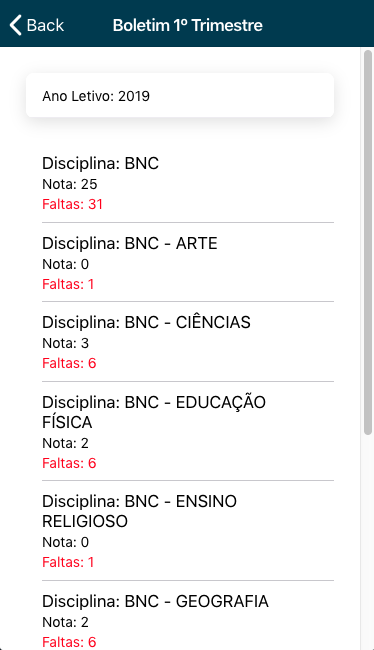
\includegraphics[width=6cm]{resources/prints_app/boletim.png}} % leia abaixo
    	\label{figura:login}
    	\caption*{Fonte: O Autor.}
    \end{minipage}
\end{figure}

\begin{figure}[H]
    \caption{Listagem de frequências por trimestre.}
	\centering % para centralizarmos a figura
	\shadowbox{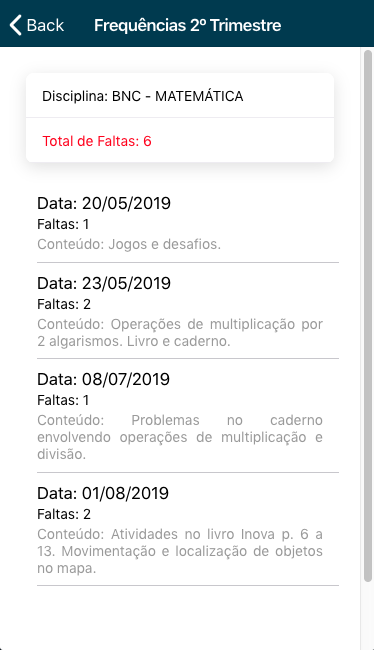
\includegraphics[width=6cm]{resources/prints_app/frequencias.png}} % leia abaixo
	\label{figura:login}
	\caption*{Fonte: O Autor.}
\end{figure}

\subsubsection{Web Service Restful}

A implementação do Web Service foi realizada utilizando a ferramenta Netbeans 11.1,

\begin{table}[H]
	\centering
	\caption{Mapeamento dos serviços do Web Service.}
	\renewcommand{\arraystretch}{1.5}
	\begin{tabular}{>{\centering}m{1.8in} >{\centering}m{0.5in} >{\centering}m{1.2in} >{\centering\arraybackslash}m{2.0in}}
	    \hline
		\multicolumn{1}{c|}{\textbf{URI}} 
		& \multicolumn{1}{c|}{\textbf{Método}}
		& \multicolumn{1}{c|}{\textbf{Retorno}}
		& \multicolumn{1}{c}{\textbf{Descrição}}\\
		\hline
		/login & POST & - & Realiza login através das credenciais do usuário \\
		/aluno/alun/\{id\}/\{ano\} & GET & List<Aluno> & Busca dados de um aluno por id e ano letivo \\
		/resp/\{id\}/\{ano\} & GET & List<Aluno> & Busca dados de alunos por id do responsável e ano letivo \\
		/aluno/grade/\{id\} & GET & List<Aula> & Busca aulas de uma grade horária por id do aluno \\
		/ativ/\{id\}/\{per\}/\{disc\} & GET & List<Atividade> & Busca atividades avaliativas por id do aluno, período e id da disciplina \\
		/ativ/\{id\}/\{per\} & GET & List<Disciplina> & Busca disciplinas para consulta de atividades avaliativas por id do aluno e período \\
		/aluno/boletim/\{id\}/\{per\} & GET & List<Boletim> & Busca boletins por id do aluno e período \\
		/freq/\{id\}/\{per\}/\{disc\}/total & GET & List<Frequencia> & Busca frequências por id do aluno, periodo e id da disciplina \\
		/freq/\{id\}/\{per\}/\{disc\}/total & GET & Integer & Busca total de frequências por id do aluno, periodo e id da disciplina \\
		/freq/\{id\}/\{per\} & GET & List<Disciplina> & Busca disciplinas para consulta de frequências por id do aluno e período \\
		/freq/\{id\}/\{per\}/total & GET & Integer & Busca total de faltas por id do aluno e período \\
		/cale/\{ano\} & GET & List<DiaCale> & Busca dias do calendário acadêmico por ano letivo \\
		/usuario/msg/\{id\} & GET & List<Mensagem> & Busca mensagens pelo id do usuário \\
		/aluno/classify/\{id\} & GET & double[] & Busca recomendação de área de aptidão com base no Novo Ensino Médio \\
		\hline
	\end{tabular}
	\label{tabela:app_organizacao}
	\caption*{Fonte: O Autor.}
\end{table}

\subsection{Testar}

\subsection{Implantar}

\section{Módulo de Recomendação baseado em Redes Neurais}

A Implementação do módulo baseado em redes neurais foi implementada utilizando a biblioteca Weka, 

O processo de treinamento da rede foi realizado utilizando 

\section{Avaliação do Software}

Foi realizado avaliação do software construído através de pesquisa realizada com alunos do ensino médio integrado do Ifes Campus Cachoeiro de Itapemirim. 

\begin{figure}[H]
	\caption{Avaliação do aplicativo por alunos do ensino médio do IFES Campus Cachoeiro.}
	\centering % para centralizarmos a figura
	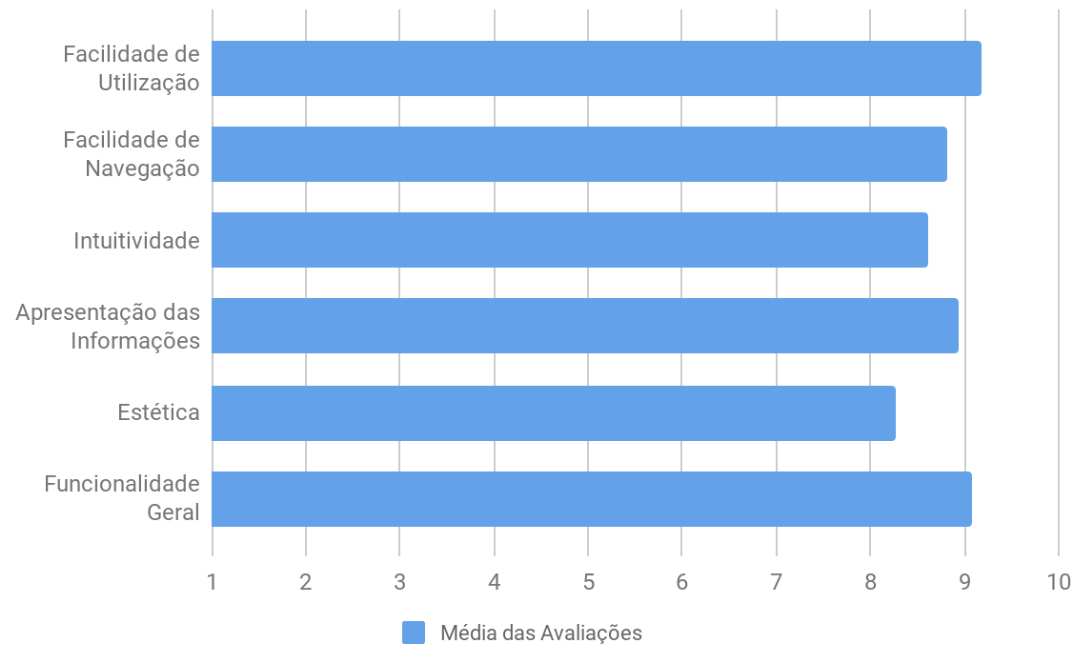
\includegraphics[width=15cm]{resources/pesquisa_avaliacao.png} % leia abaixo
	\label{figura:avaliacao}
	\caption*{Fonte: O Autor.}
\end{figure}